\documentclass[11pt,twoside]{article}
\usepackage[utf8]{inputenc}
\usepackage[margin=1in]{geometry}
\usepackage{titlesec}
\usepackage{parskip}
\usepackage{fancyhdr}
\usepackage{amsmath, amssymb}
\usepackage[round,sort&compress]{natbib}
\usepackage{tikz}
\usetikzlibrary{positioning, arrows.meta, fit, backgrounds}
\usepackage{hyperref}

% Approximation of JMLR style parameters
\setlength{\parindent}{0pt}
\setlength{\parskip}{0.3em}
\titlespacing*{\section}{0pt}{0.6em}{0.3em}
\titlespacing*{\subsection}{0pt}{0.5em}{0.2em}

\pagestyle{fancy}
\fancyhf{}
\lhead{\footnotesize STAT8101}
\chead{\footnotesize \href{http://www.cs.columbia.edu/~blei/teaching.html}{Invariance, Causality, and Applications}}
\rhead{\footnotesize \href{http://www.cs.columbia.edu/~blei/}{David M. Blei}}
\cfoot{\thepage}

\begin{document}
\vspace*{-1.5cm}
\begin{center}
{\Large \textbf{Reader Report: Week 10}} \\
\vspace{0.2em}
{\large Bayesian Optimization and Adaptive Experimental Design} \\
\vspace{0.3em}
Daniel Hardesty Lewis (\texttt{dl3645}) $\cdot$ Spring 2026
\end{center}
\vspace{-1.5em}
\thispagestyle{fancy}

\section*{Summary}
Bayesian Optimization (BO) formalizes global optimization of expensive, black-box functions via adaptive experiments. A probabilistic surrogate (e.g., Gaussian Process) tracks belief over the objective; an acquisition function (e.g., Expected Improvement) dictates queries $x_t$. BO is causal optimization only if queries represent interventions targeting interventional estimands (e.g., $\mathbb{E}[Y \mid do(A=a)]$). It evaluates expensive objectives via probabilistic surrogates, bypassing structural equations.

\section*{Critique}
The leap from synthetic controls (SC) and invariant causal prediction to Bayesian Optimization bridges evaluating historical policy interventions and dynamically prescribing new ones. As detailed by \citet{shi2022sc}, SC weights and causal identifiability rely on fine-grained individual potential outcomes, independent causal mechanisms, and structural conditions ensuring stability, overlap, and similarity across selected donors (Theorem 1). In urban models, scaling from individual resident opinions to neighborhood-level protest events suggests SC's linear structure arises from expectation and aggregation, not linear individual mechanisms. This ensures identifiability is a rigorous property of target-donor composition, not mere computational convenience.

Using BO in social domains introduces tension. Under domain generalization, the environment $e \in \mathcal{E}$ indexes a sampling distribution or regime; it is not typically an active choice variable. If distributions undergo structural mechanism shifts (opposed to covariate shifts under stable mechanisms), the GP surrogate's stationary covariance miscalibrates. Incorporating causal structure directly into probabilistic models (using Causal Bayesian Optimization \citep{aglietti2020cbo}, leveraging causal graphs and $do$-calculus to weigh observation and intervention) is vital to deploying adaptive design across unstable geographic regimes.

\section*{Questions}
\begin{enumerate}
    \item When extending BO to causal domains, confounding (the mismatch between $\mathbb{E}[Y \mid X=x]$ and $\mathbb{E}[Y \mid do(X=x)]$ due to unmeasured common causes) cannot be resolved merely by decomposing epistemic variance and aleatoric observation noise in a GP posterior. How can dynamic BO models integrate identification assumptions (e.g., back-door adjustments or instrumental variables) before utilizing posterior variance for exploration?
    \item If the underlying structural causal model shifts dynamically over time (e.g., a policy intervention alters the true mechanisms rather than just inducing covariate shift), how do formal nonstationary frameworks (like time-varying GP bandits \citep{bogunovic2016time} or Dynamic Causal Bayesian Optimization \citep{aglietti2021dcbo}) track the drifting optimum without manually re-initializing the GP prior?
\end{enumerate}

\newpage
\vspace{1em}
\hrule
\vspace{1em}
\section*{Project Update: Zoning Policy as Adaptive Experimental Design}
\thispagestyle{empty}

\begin{abstract}
My project formalizes the prediction of protest petitions against housing developments as an Empirical Risk Minimization (ERM) problem subject to spatial and temporal domain shifts. Building on our invariant causal prediction framing, this update explores framing municipal rezoning interventions not as static treatments, but as an ongoing \textit{constrained Bayesian Optimization} problem managed by the city council.
\end{abstract}

\section*{The Questions (What, Why, How)}
\textbf{What:} Can we model municipal zoning pipeline approvals as a structured Bayesian Optimization process where planners adaptively test spatial policy interventions corresponding to well-defined potential outcomes under an unknown NIMBY-resistance constraint? \\
\textbf{Why:} Standard retrospective analyses evaluate spatial shocks statically. However, cities operate sequentially: granting density bonuses, observing noisy protests, and calibrating future approvals. By defining the city's behavior through BO constraint satisfaction algorithms (e.g., SAFEOPT) guaranteeing safe exploration, we can simulate optimal development trajectories. \\
\textbf{How:} Implement a constrained Gaussian Process surrogate structured around a causal SCM. We define the action node as the zoning policy ($A$), the outcome as realized housing units ($Y$), the protest hazard as petition occurrence ($P$), and index unobserved confounders as $U$, distinguishing them from regime $e \in \mathcal{E}$. The constrained causal objective under regime $e$ is:
\[
    \max_{a \in \mathcal{A}} \ \mathbb{E}[Y \mid do(A=a), U, e] \quad \text{s.t.}\quad \Pr(P=1 \mid do(A=a), U, e) \le \delta
\]

\begin{figure}[h]
\centering
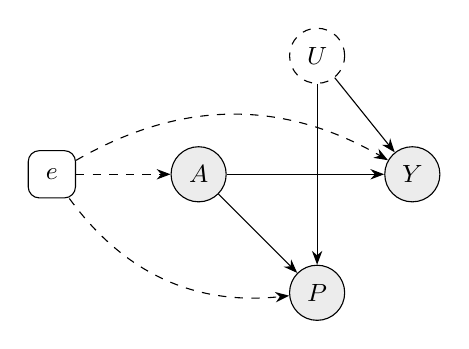
\begin{tikzpicture}[
    node distance=1.5cm and 1.5cm,
    obs/.style={draw, circle, fill=gray!15, minimum size=0.7cm, font=\small},
    latent/.style={draw, circle, dashed, minimum size=0.7cm, font=\small},
    regime/.style={draw, rectangle, rounded corners, minimum size=0.6cm, font=\small},
    >={Stealth[length=5pt]}
]
  \node[obs] (A) {$A$};
  \node[obs, right=2cm of A] (Y) {$Y$};
  \node[obs, below right=1cm and 1cm of A] (P) {$P$};
  \node[latent, above right=1cm and 1cm of A] (U) {$U$};
  \node[regime, left=1.2cm of A] (e) {$e$};

  \draw[->] (A) -- (Y);
  \draw[->] (A) -- (P);
  \draw[->] (U) -- (Y);
  \draw[->] (U) -- (P);
  
  \draw[->, dashed] (e) -- (A);
  \draw[->, dashed] (e) to[bend left=30] (Y);
  \draw[->, dashed] (e) to[bend right=30] (P);
\end{tikzpicture}
\caption*{\footnotesize Causal DAG for zoning policy optimization. Solid nodes are observed; the dashed node $U$ denotes unobserved confounders. The boxed regime node $e$ uses dashed arrows to indicate that structural mechanisms (not just marginal distributions) shift across geographic or temporal regimes, motivating the DCBO formulation.}
\end{figure}

\section*{Mathematical Description \& Strategy}
We form a sequential decision-making pipeline where action $a_t$ maximizes yield without violating defined safety margins. To ensure mathematical consistency for probabilistic constraints, we define a real-valued latent safety margin $g(a)$ instead of directly assigning a GP to a bounded probability. The surrogate models are Gaussian Processes:
\begin{align*}
    f(a) &\sim \mathcal{GP}(m_f(a), k_f(a, a')) \quad \text{(Housing Yield Objective)} \\
    g(a) &\sim \mathcal{GP}(m_g(a), k_g(a, a')) \quad \text{(Latent Protest Safety Margin)}
\end{align*}
We map the latent margin to a protest probability via a link function $\pi(a)=\sigma(g(a))$, enforcing feasibility as $g(a) \le 0$. Denoting the current best feasible observation (incumbent) as $f^*$, the Expected Improvement (EI) evaluates the expected gain:
\[
    \alpha_{\text{EI}}(a) = \mathbb{E}[\max(0, \ f(a) - f^*) \mid \mathcal{D}_t]
\]
which has a closed form driven by the GP posterior mean and variance \citep{garnett2023bayesian}. Assuming independence, Constrained EI factorizes multiplicatively: $\alpha_{\text{CEI}}(a) = \alpha_{\text{EI}}(a) \cdot \Pr(g(a) \le 0)$. Housing yield and protest risk are fundamentally correlated. If independence fails, joint modeling of constraints (e.g., multi-task GPs) is necessary. Because zoning approvals are noisy and outcomes are delayed, we must employ algorithms explicitly addressing noisy constraints (e.g., Safe Exploration via SAFEOPT \citep{sui2015safeopt}), providing high-probability safety guarantees rather than evaluating deterministic boundaries.

\section*{Integration with Current SCM Framing}
This formulation enhances the SCM structures within my draft \citep{peters2016icp, arjovsky2019irm, krueger2021rex, shi2022sc}. Rather than a flat concept shift assumption, we formally model the 2022 Austin municipal election turnover as a structural change point altering the causal graph's parameters under Dynamic Causal BO (DCBO) \citep{aglietti2021dcbo}. Instead of continuous drift, this change-point formalization allows us to analyze how the discrete policy handover structurally modified the mechanisms determining protest hazards, resetting the surrogate belief over the interventional estimand.

\section*{Next Steps}
I will begin mapping the 7,074 historical discretionary zoning cases into a simulated sequential optimization pathway, building a post-hoc analysis to see if the historical sequence of council approvals was systematically more exploratory or exploitative than an idealized safe BO algorithm \citep{sui2015safeopt}.

\vspace{-0.5em}
{\scriptsize
\setlength{\bibsep}{0pt}
\bibliographystyle{plainnat}
\bibliography{references}
}
\end{document}
